\chapter{归纳不变式自动生成工具的实现}\label{chap:implementation}

本章节将基于设计方案,详细介绍了归纳不变式自动生成工具的实现细节,包括模块之间的交互以及模块的具体实现。

\section{总体实现}
主要包括输入模块、候选不变式检验模块、候选不变式生成模块和非功能模块。

输入模块主要负责接收用户传入的\TLA 规约文件,配置信息等,将这些信息存储以供后续使用。
对\TLA 规约文件,利用tla2sany工具将其转换为抽象语法树,并通过遍历抽象语法树,获取规约文件中常量、变量和谓词的定义。

非功能模块包括日志功能,计时功能,报错信息等,这些功能伴随着系统每个行为,为开发人员和用户提供更多信息,方便调试和使用。
日志模块需要以不同的记录级别记录系统运行的行为和结果,尤其是对于TLC和Apalache的调用的结果,因为是外部调用,需要格外关注。
计时模块需要记录系统运行的总时间和每个部分分别运用的时间。

\section{候选不变式检验模块}

候选不变式检验模块主要的职责是对生成模块的生成的候选不变式的正确性,给出的候选归纳不变式的递归性,以及对新生成不变式的独立性进行判断。

候选不变式检验模块接入了TLC和Apalache,用户可以选择其一对生成的候选不变式进行验证。
TLC 和 Apalache 是两个常见的面向\TLA 规约的模型检查工具(model checker),可以使用相似的配置文件对规约进行验证,
但是,两者的结果输出格式不同,需要做分别处理。

由于Apalache需要用户对协议中的变量和常量做出类型的注释,因此,目前能够提供的测试集中大多数的规约都无法使用Apalache进行验证。
在系统实现时,我们默认状态下使用TLC作为系统的模型检查器。
当然,在条件允许时,用户可以设置系统的参数来使用Apalache作为系统的模型检查器。

在检验候选的不变式和归纳不变式时,如果出现反例,无论是对候选不变式的反例,还是对归纳不变式的归纳反例,都应该提取出来,返回给生成模块。

\subsection{model checker的配置文件和运行选项}

对于图\ref{fig:client_server}中的规约,TLC 和 Apalache 会使用默认的配置文件进行验证,
即以 $\text{INIT}$为初始状态,$\text{NEXT}$ 为状态转移关系,在状态变化的过程中验证 $\text{Safe}$ 安全属性的正确性。
用户也可以指定使用其他配置文件,以验证从不同状态出发和不同状态转移条件下的用户定义的不变式的成立与否。
比如说需要验证的不变式,可以放在$\text{INVARIANT}$ 字段下。
对于一些常量,用户也可以通过配置文件$\text{CONSTANTS}$字段进行定义。
一个典型的TLC配置文件如下:
\begin{lstlisting}[caption={TLC 配置文件}]
INIT Init
NEXT Next

INVARIANTS Inv_0 Inv_1 Inv_2

CONSTANTS
Node = {n1,n2,n3}
Request = {r1,r2}\nResponse={p1,p2}
n1 = n1
n2 = n2
n3 = n3
r1 = r1
r2 = r2
p1 = p1
p2 = p2
\end{lstlisting}
我们可以简单的理解为,模型检测器可以判断$\text{INIT} \wedge \text{NEXT} \vDash \text{INVARIANT}$ 是否成立。
在不成立时,模型检测器会给出一个状态的链接,展示系统状态如何从初始状态转移到不满足不变式的状态。

我们希望TLC和Apalache为我们验证生成模块生成的候选不变式的正确性,独立性和与已有不变式合取结果的递归性。
在验证过程中,我们希望模型检查器能够输出验证结果,以及验证过程中的反例(Counterexample)。

验证不变式的正确性是验证这三种性质中最为简单的。
只需要将需要验证的候选不变式放入$\text{INVARIANT}$字段中,然后运行模型检查器即可。
如果没有报错,说明候选不变式在规约的有限实例上保持布尔值为真。

由于候选的归纳不变式是由一系列引理不变式和安全属性合取而来,且每一个合取子式都满足$\text{Init} \wedge \text{Next} \vDash \text{Lemma}$,
所以候选归纳不变式自然满足引理\ref{con:init}和\ref{con:safety}。
验证候选的归纳不变式的递归性质时,我们只需要验证引理\ref{con:inductive}的正确性,我们需要验证归纳不变式在状态转移后依然成立。
在此过程中,模型检查器弹出的报错就是归纳反例。

验证不变式的独立性是验证这三种性质中最为困难的。
检查不变式的独立性就是检查新生成的引理不变式是否能杀死(eliminate)候选的归纳不变式的归纳反例。
借助TLC,我们将系统的初始状态设置为这些归纳反例的状态之一,也就是将$\text{INIT}$ 设置为这些归纳反例状态的析取。
然后看在这些状态下,哪些新生成的引理不变式不成立。不成立便能代表它们能够杀死对应的归纳反例。
在操作中,我们需要用变量记录下这些引理不变式的值。
使用TLC的\textbf{"-dump"}选项将每个状态下的变量值输出到文件中,然后解析这些文件,找到能够杀死归纳反例的引理不变式。
如果归纳反例太多,会导致TLC计算状态转移关系的时间过长,状态转移图过于复杂。
尽管可以通过\textbf{"-workers"}选项添加TLC调用的线程数量,但是也收效甚微。
因此将归纳反例分组,分别使用一个线程对每一组归纳反例进行验证,可以有效减少验证时间。

但是这种做法并不充分,还需要通过$\text{IndCand} \wedge \text{Next} \nvDash \text{Lemma}$的结果来确认新引理不变式的独立性。

我们需要将新生成的不变式放到一个新的文件中,并使用关键字\textbf{EXTENDS} 将原有规约中的定义引入。
这样,我们就可以在新的文件中使用原有规约中的定义,和引入生成模块生成的候选不变式。
由于新的\TLA 文件中有着相似的结构,在验证同一个性质时,配置文件是可以复用的。
所以我们在系统运行之初就定义好配置文件中的内容,并写入硬盘供TLC/Apalache使用。

在使用TLC验证时,我们还需要关注诸多选项。
\textbf{"-config"}是我多样化使用TLC和apalache的关键,通过这个选项,我们可以指定TLC和Apalache的配置文件,以检验不变式的不同性质。
\textbf{"-deadlock"}选项用于检查是否存在死锁状态,如果选择了这个选项,那么TLC就不会检验死锁。
由于我们的目的是检验不变式的一些性质,所以我们不需要检验死锁,并选择了这一选项。
\textbf{"-continue"}选项揭示了TLC在检测出错误后是否继续运行,为了得到更多的反例,我们需要使用这个选项。

\subsection{model checker 的调用和结果解析}
本项目的代码主要基于Python实现,然而不论是TLC还是Apalache,都是Java实现的模型检查器,且没有可以直接调用的Python接口。
因此,我们需要通过Python的subprocess库来调用Java程序,并通过解析Java程序的命令行输出结果来获取验证结果。
在验证不同性质的时候指定好不同的配置文件并调整好不用的运行参数。

对于结果的解析,主要是将TLC或Apalache的输出结果进行解析,去除无用的信息,将有用的信息交给生成模块,以便强化学习模块调整策略,提高生成的候选不变式的正确性。
TLC和Apalache尽管两者有着不同的输出格式,但是它们的功能其实是一致的,都是将出现不变式错误时的状态,以及前序状态,也就是错误轨迹(error trace)。
错误轨迹的每一个节点都是一个状态,表达的是在这个状态下,各个变量的值。
TLC会以析取范式的形式将各个变量的值表达出来,而Apalache默认使用的json文件格式,将各个变量的值以键值对的形式表达出来。
我们需要将这些信息解析出来,以便强化学习模块能够理解这些信息,调整生成的候选不变式。

不变式反例和归纳反例有着相似的作用,都是用于提示用户或者生成模块,哪些状态下,不变式或者归纳不变式不成立。

\begin{figure}[htb]
	\centering
	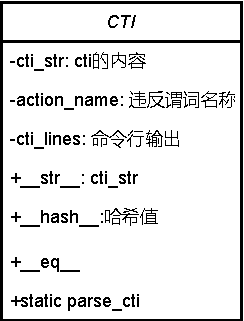
\includegraphics[width=0.3\textwidth]{figures/class_cti.pdf}
	\caption{CTI 类信息}
	\label{fig:class_cti}
\end{figure}
类CTI的信息如图\ref{fig:class_cti}。在模型检测器检测去不变式或者归纳不变式的错误时,
通过类CTI中的静态方法\textbf{parse\_cti},可以将错误轨迹提取出来,生成多个不同的cti对象。

CTI类反应的是一个状态,在这个状态下,所有变量的值存储在\textit{cti\_str}字段中。
从这个状态出发,系统可以运行一个状态,这个状态下,给出的候选归纳不变式不成立。
一个TLC输出的错误轨迹如代码段\ref{lst:cti_cmd}。
其中(State\ 1, State\ 2)就是图\ref{fig:ind-cti}的一个归纳反例,CTI类存储的是State\ 1的状态信息,cti.action\_name 对应于ReceiveResponse,
cti.cti\_str存储的是State\ 1的状态信息。

\begin{lstlisting}[caption={反例的命令行输出}, label={lst:cti_cmd}]
Simulation using seed 4257 and aril 0
Error: Invariant InvStrengthened is violated.
Error: The behavior up to this point is:
State 1: <Initial predicate>
/\ request_sent = {<<n2, r1>>, <<n3, r2>>}
/\ match = {<<r1, p1>>, <<r1, p2>>, <<r2, p1>>, <<r2, p2>>}
/\ response_received = {<<n2, p2>>}
/\ response_sent = {<<n1, p1>>, <<n1, p2>>, <<n2, p1>>, <<n3, p1>>}

State 2: <ReceiveResponse line 31, col 5 to line 33, col 53 of module client_server_ae>
/\ request_sent = {<<n2, r1>>, <<n3, r2>>}
/\ match = {<<r1, p1>>, <<r1, p2>>, <<r2, p1>>, <<r2, p2>>}
/\ response_received = {<<n1, p2>>, <<n2, p2>>}
/\ response_sent = {<<n1, p1>>, <<n1, p2>>, <<n2, p1>>, <<n3, p1>>}	
\end{lstlisting}

CE类有着和CTI类相似的结构,不同的是,CE类更关注那个使得不变式不成立的状态。
CE类对应的状态都是系统正常运行时可达的状态,而CTI类对应的状态是则全部不是系统正常运行时可达的状态。


\section{候选不变式生成模块}

生成模块是本项目的关键,它负责生成候选不变式,检验模块是为生成模块服务的。
不同于以往的归纳不变式生成工具,使用随机枚举的方式生成候选不变式,我们引入强化学习来提高我们枚举的效率和成功率。
强化学习是一种通过智能体和环境的交互,智能体通过观察环境的状态,采取行动,获得奖励,来学习如何在环境中获取最大的奖励。
强化学习的智能体通过观察检验模块对已经生成的候选不变式和候选归纳不变式的验证结果,调整生成候选不变式的策略,提高生成候选不变式的效率和准确率。

强化学习框架是本项目的核心,它负责生成候选不变式,检验模块是为生成模块服务的。
\rltla 核心逻辑是通过提供必要的信息和反馈,让强化学习智能体选择合适的种子,将它们组合起来,生成引理不变式的候选。
一个强化学习框架可以分为环境和智能体两个部分,分别是环境和智能体。
图\ref{fig:agent_env}简单地介绍了本文中的强化学习框架,描述了智能体和环境交互,不断生成候选引理不变式的大致过程。
\begin{figure}[h]
	\centering
	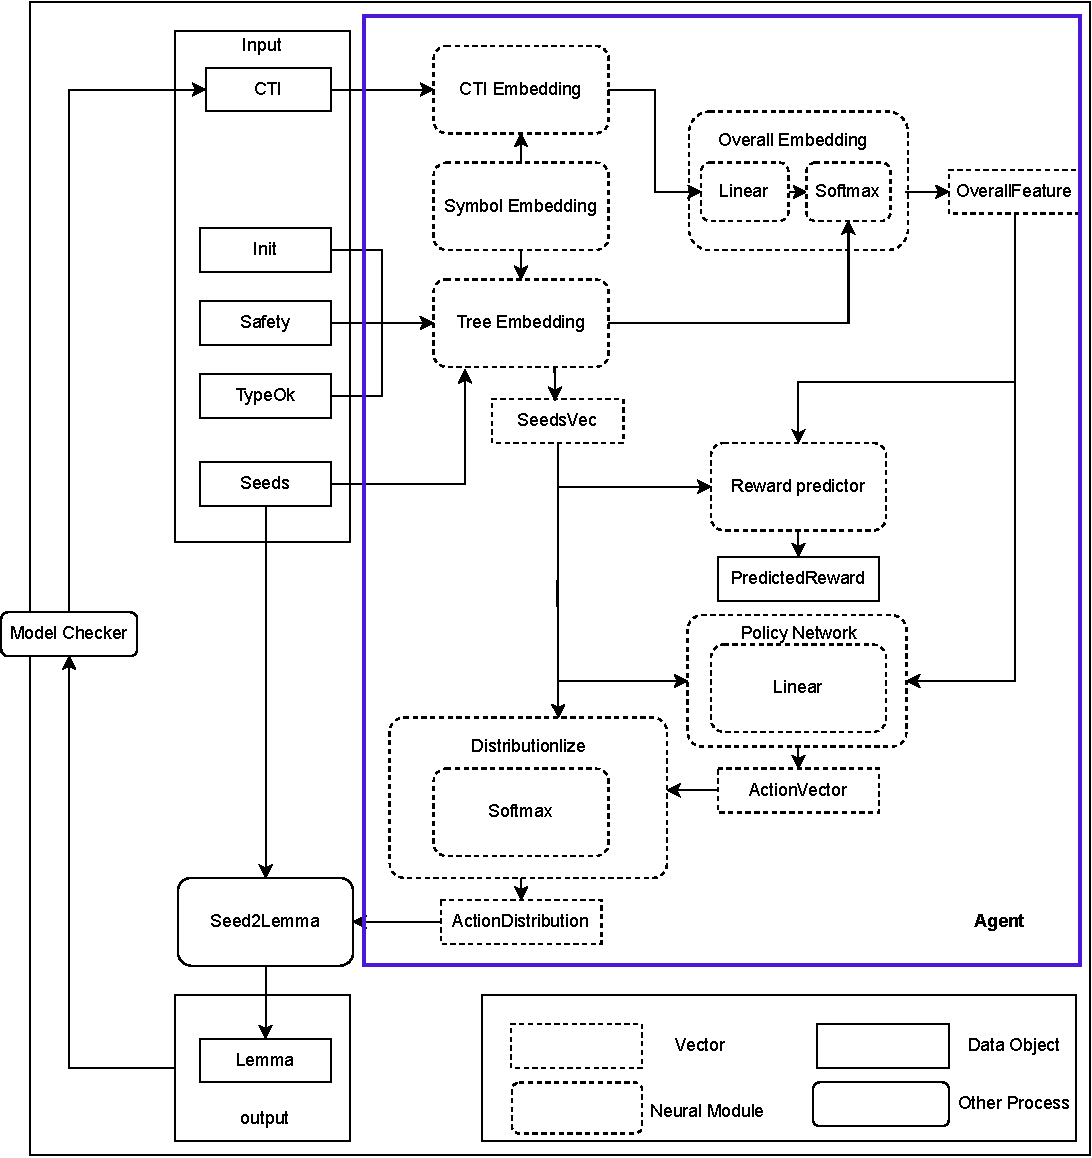
\includegraphics[width=0.8\textwidth]{figures/agent_env.pdf}
	\caption{\rltla 强化学习框架}
	\label{fig:agent_env}
\end{figure}

\subsection{强化学习环境}

环境模型是环境在强化学习中的数学表示,包含了环境中的重要信息,和对智能体的动作做出反馈。
本文中,环境给智能体提供的内容包括输入部分,也就是\TLA 规约本身和用于提供给智能体选择的种子、以及在每轮循环中的反馈,即反例和归纳反例。
这些信息足够作为智能体生成候选不变式的提示。

对于反例和归纳反例的介绍,我们在候选不变式检验模块中已经有所介绍,这里不再赘述。

输入部分,主要目的是存储和必要的数据和约束强化学习智能体的行为,使得其所能采取的行为能生成的候选不变式都必须符合基本的语法。

输入部分包括\TLA 规约文件,以及以json形式存储的对规约的配置文件。
\TLA 规约文件是生成归纳不变式的基础和目标,规约文件和相关的配置使\rltla 能够运行一个有限的实例。
基于有限实例的运行数据,也就是各个可达的状态信息,\rltla 可以以此为依据生成引理不变式和组成归纳不变式。
对图\ref{fig:client_server}中的规约,关于配置文件的具体信息,我们在第\ref{chap:run-analysis}有具体展示。
配置文件中包括生成规约有限实例的参数,主要包括常量的范围和对常量的定义,类型限制(typeok)和安全属性(Safety)。
preds 字段下是生成候选不变式的种子(seed)。quants 字段下存储的是默认的量词。
生成的候选不变式就是按照语法规则,组合种子和量词,生成符合语法的候选不变式。

环境部分还包括对智能体动作的奖惩机制,奖惩机制是智能体在环境中学习的重要手段。
基于智能体给出的不同的不变式,环境需要给出不同的奖惩。
表\ref{tab:award_punish}给出了具体的数值设置。
\begin{table}[!htbp]
	\centering
	\caption{奖励与惩罚的情况设置}
	\renewcommand\arraystretch{1.4}
	\begin{tabular}{p{0.14\textwidth}p{0.1\textwidth}p{0.3\textwidth}p{0.3\textwidth}}
		\toprule
		\textbf{类型}&\textbf{程度}&\textbf{情况}&\textbf{取值}\\
		\midrule
		奖励&very&通过归纳不变式的检测&101\\
		奖励&little&通过蕴含检测但没能通过归纳
		不变式检测&消除的CTI数量(被归一化到区间[1,100])\\
		惩罚&little&没有通过蕴含检测&-1\\
		惩罚&medium&不变式检测超时&-5\\
		惩罚&very&没有通过不变式检测&违反的状态数量(被归一化到区间[-100,-6]) \\   
		\bottomrule
	\end{tabular}
        \label{tab:award_punish}
\end{table}

\subsection{强化学习智能体}
智能体是强化学习的核心组件。智能体是学习和决策的主体。它通过与环境的交互,不断更新自己的策略(policy),以获得最大的奖励。
这个过程中有三个主要步骤:感知环境的状态,选择行动,获得奖励并更新策略。

智能体通过环境中状态的数据来感知环境,这些数据包括规约信息,种子信息和当前的CTI信息。
在接受这些数据前,需要先对数据进行预处理,将数据从高维或稀疏数据转换为低维、密集向量。这个动作叫做数据嵌入,是强化学习中的一个重要步骤,
可以简化数据结构,使其在机器学习模型中更易于处理和分析。嵌入的目的在于捕捉数据的语义或结构信息,同时减少数据的维度和复杂度。
本文在此选择的是LSTM(Long Short-Term Memory)的嵌入方法,LSTM是一种特殊的递归神经网络,专门设计用来解决普通RNN在处理长序列数据时存在的梯度消失和梯度爆炸问题,
因此适合作为数据嵌入的方法。

选择行动则表示的是智能体在当前状态下,根据策略选择行动的过程。在本文中,智能体的行动是选择种子,将种子组合成候选不变式。
智能体的策略表示智能体在不同的状态下,选择不同行动的概率,策略选择的结果直接指导了智能体的行为。
值函数用于评估状态-动作对的“价值”,即从该状态或状态-动作对开始,智能体在未来期望获得的累积奖励。
通俗地说,值函数的目的是评估智能体在某一个状态下采取某一个行动的好坏。

\textit{PolicyNetwork}和\textit{RewardPredictor}是具体实现策略和值函数的网络模型。
\textit{PolicyNetwork}的输入是系统的状态,输出是动作的概率分布。
它接受了程序的总体特征和seeds的嵌入,得到 action\_vector,再将其放到\textit{Distributionlize} 中进行归一化处理,
得到概率分布action\_distribution,用来指导seed的选择。
\textit{RewardPredictor}在奖励稀疏时十分有用,它将输入的状态向量和整体特征向量进行拼接,经过线性层逐层地提取特征,并把预测的奖励值投影到奖励值范围中,输出reward值。
在智能体采取行动后,奖励预测器还会根据实际奖励更新自己的参数,以提高奖励预测的准确性。
本文的奖励值范围是[-10, 10]。

action\_vector对应于对种子的选择。强化学习智能体选择好种子,然后交给Seed2Lemma模块,组合上量词,从而生成候选不变式。每个种子都会取其本身和取其否定并组成多个候选不变式。
这里不需要智能体选择种子或其否定,主要为了降低智能体处理问题的难度。

\begin{align}
	&\text{StrictLoss} = - \frac{1}{N} \sum_{i=1}^{N} log\_softmax(\text{action\_distribution}) \cdot \text{sd}_i \cdot \gamma \label{con:strictloss} \\
	&\text{r} = \left[ \text{f} \cdot \text{discounter}^{n-1}, \ldots , \text{f} \cdot \text{discounter}^1, \text{f} \cdot \text{discounter}^{0} \right] \label{con:r}\\
	&\text{CELoss}_i = -q_{i} \log(p_{i}) \label{con:celoss} \\
	&\text{RewardLoss} = \frac{1}{N} \sum_{i=1}^{N} (\text{r}_{i} - \text{r}_{i-1}) \cdot \text{CELoss}_i \label{con:rewardloss} \\
	&\text{MSELoss} = \frac{1}{N} \sum_{i=1}^{N} (\hat{r}_i - r_i)^2\label{con:mse} \\
	&\text{Total Loss} = \text{Strict Loss}+\text{RewardLoss}+\text{MSELoss} \label{con:totalloss}
\end{align}

智能体在采取每个行动后,除了得到环境的状态信息,包括反例或者归纳反例和候选归纳不变式的状态,还会得到奖惩值和调整系数,这两个参数用于调整智能体的策略。
智能体会计算每轮采取的行动的损失值,并通过\textit{backward}方法向后传播给模型,更新模型的参数。
损失值有三个度量维度,分别为严格性损失(Strict Loss, \ref{con:strictloss}),预测损失(Prediction Loss, \ref{con:rewardloss})
和均方损失(MSE Loss, \ref{con:mse}),其总和为总损失\ref{con:totalloss}。
表达式中,$\text{N}$表示每次选择的种子数量 $\text{sd}_i$表示每个种子被选择的概率分布。
环境的反馈中给出了调整系数$\gamma$,调整系数是用于调整严格性损失在总体损失中的占比,$\text{f}$ 则是环境给出的具体奖惩值。
$\text{p}$和$\text{q}$ 分别为$\text{action\_distribution}$的输出概率分布和目标概率分布。
三个维度的损失组成总体损失,总体损失反应了智能体做出的决策优劣,指导做出下一轮决策。

